\documentclass[hyp, 12pt]{socreport}
\usepackage{fullpage}

\usepackage{url}
\usepackage{amsmath,amsthm,amsfonts}
\usepackage{algorithm,algorithmic}
\usepackage[dvips]{color}
\usepackage{algorithm,algorithmic}
\usepackage{graphicx}
\usepackage{CJKutf8}
\usepackage{multicol}
\setlength{\columnseprule}{0.5pt}
\setlength{\columnsep}{20pt}

\usepackage{tikz}
\usetikzlibrary{trees}
\usetikzlibrary[positioning]
\usetikzlibrary{calc}
\usetikzlibrary{decorations.pathmorphing}
\usetikzlibrary{fit}
\usetikzlibrary{backgrounds}
\tikzstyle{level 1}=[level distance=4cm, sibling distance=3.5cm]
\tikzstyle{level 2}=[level distance=4cm, sibling distance=2cm]
\tikzstyle{bag} = [text width=4em, text centered]
\tikzstyle{end} = [circle, minimum width=3pt,fill, inner sep=0pt]
\tikzstyle{fork} = [circle, minimum width=3pt,fill, inner sep=0pt]

\begin{document}
\pagenumbering{roman}
\title{Citation Provenance}
\author{Heng Low Wee \\ (U096901R)}
\projyear{2011/12}
\projnumber{H079820}
\advisor{A/P Min-Yen Kan}
\deliverables{
	\item Report: 1 Volume
	\item Source Code: 1 DVD}
\maketitle
\begin{abstract}
\paragraph{}
We investigate a new task in citation analysis, {\it citation provenance}, to locate the location of the cited information that justifies a citation. We describe the challenges in collecting annotations for our training set, and present a two-tier approach in tackling this problem. We adopted some features used in Citation Classification and Information Retrieval tasks and with them we differentiate citations that referred to the whole paper in general ({\it general}) versus ones the cited specific claims, evidence or parts of the paper ({\it specific}) and then given that a citation is {\it specific}, locate the cited information in the cited paper. The first tier ({\it GvS}) obtained a promising accuracy of $0.786$ in cross-validation evaluation and in terms of $F_1$ score the second tier ({\it LocateProv}), at $0.90$, performed about $25\%$ better than the baseline.

\begin{descriptors}
	\item H. INFORMATION SYSTEMS
\end{descriptors}
\begin{keywords}
	citation analysis, citation provenance, source of citation, citation classification
\end{keywords}
\begin{implement}
\begin{flushleft}
\hspace{5 mm}Software: Python, NLTK\footnote{http://nltk.org/}, scikit-learn\footnote{http://scikit-learn.org/} \nocite{scikit-learn}\\
\hspace{5 mm}Hardware: MacBook Pro, Intel Core 2 Duo 2.4GHz, 4GB Memory.
\end{flushleft}
\end{implement}
\end{abstract}

\begin{acknowledgement}
\paragraph{}
I would like to express my gratitude to all the volunteer participants from the NUS WING group for participating in my pilot annotation tests. I thank them for testing my annotation scheme, and appreciate the feedback that improved my project.

\paragraph{}
Congrats to the \url{CodeForScience} team from WING NUS, consisting of Jin Zhao, Tao Chen, Eric Yulianto Ang and myself for having emerged the winners for the competition with our prototype application CitWeb that integrated our projects -- Citation Classification and Citation Provenance.

\paragraph{}
Million thanks to Jin Zhao, Tao Chen, and especially my supervisor to this project, A/P Min Yen Kan for providing their guidance during the duration of the project.
\end{acknowledgement}

\listoffigures
\listoftables
\tableofcontents

\chapter{Introduction}
\label{introduction}
\paragraph{}
In the English language, there are many words and even phrases that have multiple interpretations depending on the context. These words have multiple \textit{senses} or meanings, and are ambiguous. For instance:
\begin{enumerate}
\item She is interested in the \textit{interest} rates of the bank.
\item He developed an \textit{interest} in art.
\end{enumerate}

\paragraph{}
It is not difficult for a human to see that the word \textit{interest} has different meanings in the two sentences. We humans are able to determine the context of each sentence immediately, and hence able to identify the correct sense for the ambiguous word. A machine, however, needs to run through a series of analytical processes before it can determine the best answer. This process is termed Word Sense Disambiguation (WSD). More formally, WSD is the process of deciphering the intended meaning of an ambiguous word in a given context.

\paragraph{}
%%%From Aobo: "such as machine learning" ml is not an example of application.  machine translation?
%%% updated
WSD is a key task in Natural Language Processing. It has many applications in computational linguistics, such as machine translation, text mining and information retrieval. It can also be applied within search engines such that the search results will be more relevant, when the results have the same intended meaning as the search query.

\paragraph{}
There are four conventional types of WSD, they are:
\begin{enumerate}
\item Dictionary-based \& knowledge-based \\
This method uses formal dictionaries and lexical knowledge bases as their primary source to disambiguate senses. Dictionaries provide the definitions of the possible senses of an ambiguous word. The definitions can then be used in WSD algorithms. One example is the Lesk Algorithm \cite{lesk}, that words in a given environment (sentence, paragraph etc) will tend to share a common topic. Banerjee \& Pedersen, instead of using standard dictionaries,  used WordNet \cite{wordnet} as a sense inventory in their implementation of the Lesk Algorithm. WordNet is arranged semantically, creating an electronic lexical database that provides a rich hierarchy of semantic relations that can be exploited. The authors exploited this advantage of WordNet and integrated into the Lesk Algorithm. They found that the adapted implementation outperformed the traditional Lesk approach with double the accuracy.
%%From Chen Tao:The whole paragraph emphasizes the use of dictionaries (formal or informal), but not mention much about knowledge bases. Can I just understand that dictionaries also provide lexical knowledge? It will be better if introducing the relationship between dictionary-based and knowledge-based method.
\item Supervised \\%%From aobo : maybe need reference for this paragraph. and the first sentence is not definitely correct.
% updated
Supervised WSD uses manually sense-tagged corpora as their primary resource to perform WSD. It can be formulated as a classification problem where word senses represent classes and a classifier assigns a class to a new instance of a word. Some classifiers are the Naive Bayes, Decision Lists \cite{supervisedmethods} and Support Vector Machines \cite{svm}.
%Support Vector Machines have been known to be one of the most successful approaches for WSD because they can cope with high-dimensionality of the feature space.
\item Semi-supervised \\
This method makes use of both labeled and unlabeled data. Similarly, it refers to using multiple untagged corpora to provide concurrent information to supplement a tagged corpus.
\item Unsupervised \\
Most challenging approach among all, this method may also be related to \textit{Word Sense Induction}, where senses could be induced by analyzing words in a given text. Unsupervised methods perform WSD with minimal, or no, dependence on sense-tagged corpus. \cite{noisy} described a probabilistic approach based on the Noisy Channel Model that uses an unlabeled word corpus derived from publicly-available web pages. Their system outperformed all the unsupervised systems compared with, some of which the authors claimed that they should be classified as semi-supervised instead.
\end{enumerate}

\section{Motivation}
%%From Aobo: your contribution is the balance between efficiency and accuracy, so the motivation should mention the balance beside simply benefiting MT.
%updated
\paragraph{}
There are many WSD systems that can provide great accuracies in disambiguating words. However, most of these systems are also not publicly available, either for its applications or for further research. Also, these systems are not suitable to be deployed as real-time softwares, such as for use on mobile devices, as the size of their training models are relatively large to be suitable.

\paragraph{}
The motivation in this project, other than to encourage the usage of WSD applications, is to build WSD systems that are small, and responsive such that they are more suited to be deployed on mobile devices or web browsers.

%\paragraph{}
%The motivation in this project is its benefits when applied into bilingual translation. For instance, English to Chinese. Consider this example:
%\begin{center}
%He developed an \textit{interest} in art.
%\end{center}
%\paragraph{}
%In this context, we can see that the word \textit{interest} is more related to the word ``hobby''. So when we translate the word \textit{interest} from English to Chinese, the correct output would be \begin{CJK}{UTF8}{gbsn}兴趣\end{CJK} (a person's interest) instead of \begin{CJK}{UTF8}{gbsn}利息\end{CJK} (simple interest). Being able to translate while retaining the original context would definitely prove to be more relevant for the end-users. Furthermore, this would encourage language learning as it is simpler and more straightforward when a learner is aware of which is the correct sense to be used in a given context.

%\paragraph{}
%In this paper, however, we do not venture into the field of translating the words into a second language. Instead, we focus on studying how we can predict the word senses of ambiguous words in the English language.

%%%From Aobo: before performance indicators, a chapter explaining what your approach(DT) is and why you use this approach(DT) is needed.
% updated
\section{Goals}
\paragraph{}
In this project, we explore how we can build a system that is small, suited for real-time applications. For that, we have considered three goals to measure the performance of our system in this project. They are:
\begin{enumerate}
\item Accuracy - percentage accuracy in predicting word senses
\item Speed - time taken to predict word senses and return the results
\item Size of Model - size of the training model used by the system to predict word senses
\end{enumerate}
\paragraph{}
We intend to build a system that is meant to perform WSD on small amount of text, like a sentence. One application for such a system is a language-assistance based tool to be integrated with web browsers, like a plugin in Firefox, so that users are able to find out more information, like pronunciation and definition, about some words on the web page by selecting the text using the mouse. WSD comes into the picture as we see the need for these information to be context-relevant from where the selected text is from. However we must keep the response time small, so that we can maintain user's experience. One can imagine an user who has the habit of selecting text on web pages very often. Any language tool with slow response will be not ideal.

\paragraph{}
For that, as much as possible, we intend to keep the model size as small as possible, while retaining a reasonable level of accuracy. We want it to be speedy and responsive. Also, we hope to reduce the amount of pre-processing prior to the prediction of word senses. We believe that by including too many pre-processing features, the system would require additional supporting files that could be significant in terms of file size. 
\chapter{Related Work}
\label{Related Works}
\section{Citation Analysis}
\paragraph{}
Several authors had researched on works related to citation analysis. In these works, they could be categorised into several directions for development. One of them that has a major impact would be citation classification or similarly, the classification of citation function. This task is aimed at making sense of the rationale why the authors of a paper would cite the work of another, and thus better aid readers on understanding the key ideas presented in a paper. The reasons why authors would cite, are what was meant by the citation function. In an updated version of their paper, Teufel et al. presented an annotation scheme for annotating a citation's function \cite{teufel2009annotation}. In their scheme, citations are generalised into 4 main categories: Weak, Contrast, Postive \& Neutral. Some of these categories are further broken down into more specific sub-categories, producing a total of 12 classes for annotating citations. \cite{teufel2006automatic} had already worked on the automatic classification of citation function, utilising features extracted from the \textit{citing context}. \cite{dongensemble} presented an approach to citation classification that uses a combination of various supervised learning algorithms. Similarly, authors worked on analysing the sentiment of citations to determine the polarity of these citations. \cite{athar2011sentiment} used sentence structure based features extracted from the citing context and produced promising results.

\paragraph{}
In \cite{citation-sensitive} and \cite{csibs}, Wan and his teams worked on building a research tool that acts a reading aid for readers when browsing through scientific papers. Wan et al. investigated the \textit{literature browsing task} by conducting surveys on researchers who read scientific papers frequently to update themselves. In this initial study conducted by Wan et al., several key ideas were revealed. First, when researchers read scientific papers and see citations made by the author, their main concern, as time-constrained professionals, is whether the cited paper would be worth their time and effort, and money, to follow up on and at the same time, whether to believe in the citation. Second, readers faced the difficulty of finding the exact text that justify the citation. Third, the surveys revealed that readers found it useful if a reading tool could identify important sentences and key words in the cited paper. This study conducted by Wan et al. is based on the fundamental idea of improving the reading experience of practitioners and researchers. The goal is to save a reader's time by helping the reader make relevance judgements about the cited documents. As it is often that readers have to read up on the cited documents to gain a better insight on the current context, this task would be of relevance. The authors then developed the CSIBS based on their studies. The CSIBS tool helps reader determine whether to read on the cited papers by providing a contextual summary of the cited papers.

%Tao: Could you show the reasons of reviewing sentence alignment, that is, the connection/similarity between citation provenance and sentence alignment? 
\section{Sentence Alignment}
\paragraph{}
Aligning sentences belonging to similar documents of the same language is an important research area for tasks related to summarisation and paraphrasing. \cite{nelken2006towards} presented a novel algorithm for sentence alignment in monolingual corpora. They showed their approach, which is based on TF*IDF similarity score, produced great precision at aligning sentence, with precision score of 83.1\%. A more recent work by \cite{li2010fast} introduced a new sentence alignment algorithm called Fast-Champollion. Briefly, it splits the input text into alignment fragments and identifies the components of these fragments before aligning them using a Champollion-based algorithm.





\chapter{Problem Analysis}
\label{problemanalysis}

In the scope of our project, all citations are classified into 2 types: \textbf{General} and \textbf{Specific}. We define citations as such to be inline with our goal. That is, to be able to tell if Specific, where the cited information is in the cited document. Otherwise, the citation would be deemed General. To rid of ambiguity in our definition of a General/Specific citation, we have the following guidelines: \\ \\
\textbf{General Citations}
\begin{enumerate}
\item Authors may refer to a paper as a whole. If the author cites for a key idea, e.g. Machine Learning, and Machine Learning makes up the entire or majority of the cited paper, it is a general citation.
\item Authors may refer to a paper as a form of mentioning. The authors merely mentions the cited paper out of acknowledgement of its contributions.
\end{enumerate}
\textbf{Specific Citations}
\begin{enumerate}
\item Authors may refer to a term definition in the cited paper.
\item Authors may refer to a key idea/implementation in the cited paper. This key idea/implementation does not make up the entire cited paper.
\item Authors may refer to an algorithm or a theorem in the cited paper. This algorithm/theorem does not make up the entire cited paper.
\item Authors may refer to digits or numerical figures in the cited paper. Usually for making reference to evaluation results in the cited paper. Authors may also complement the cited paper for its promising/excellent performance.
\item Authors may quote a line/segment in the cited paper.
\end{enumerate}

\begin{figure}[h]
\label{fig:terminology}
\framebox[\textwidth]{
	\begin{tabular}{ l p{11cm}}
		\textsc{Term} & \textsc{Description}\\
		\hline
		Citing Paper & The paper that makes the citation \\
		Cited Paper & The paper that is being cited by the citing paper \\
		Cite Link & E.g. \url{E06-1034==>J93-2004}. A citation relation between a citing paper (\url{E06-1034}) and a cited paper (\url{J93-2004}) \\
		Cite String & The citation mark. E.g. Nivre and Scholz (2004), [1], (23) \\
		Citing Sentence & A sentence in the citing paper that contains the in-line citation. E.g. \textit{That algorithm, in turn, is similar to the dependency parsing algorithm of \textbf{Nivre and Scholz (2004)}, but it builds a constituent tree and a dependency tree simultaneously.} \\
		Citing Context & The block of text surrounding the citing sentence, about 2 sentences before and after the citing sentence, for providing contextual information \\
		Cited Fragment & A fragment, from a few lines to paragraphs, in the cited paper
	\end{tabular}
}
\caption{Terminologies used in this paper}
\end{figure}

In general, for \textbf{Specific} citations, we would be able to specifically extract a fragment in the cited paper that represents the source of the information mentioned in the citation itself i.e. Citation Provenance.

\section{Scope Of The Problem}
I now reduce the problem to determining whether a citation is General or Specific. If a citation is General, the reader can be directed, for example, to the Abstract section of the cited paper. If a citation is Specific, the reader can be directed to that specific paragraph or lines respectively.
%Therefore during computation, the cited document can be broken down into fragments.
If given that a citation is Specific, then there must exists a region in the cited paper that the citation refers to. For this I need to implement some ranking system that determines the location of this region.

I abstract away the problem of locating the in-line citations in a paper, and reduce the problem to only determining the type of a citation and its location. To solve the problem of locating the in-line citations, I utilize the open-source ParsCit system developed by \cite{parscit}. Conveniently, ParsCit identifies the citing sentence, together with its citing context.

\section{Modelling The Problem As Search}
In web search engines, an user enters a search query, and a search engine would use this query to search within its search domain -- millions of web pages -- and then display the best matching web pages as compared to the search query. That would be equivalent to having a search query for an entire corpus of research papers. This problem can also be modelled as a searching problem, but a reduced version as compared to web search engines.

Consider reading a paper, \url{A}. We know the citations made by \url{A}, and these cited papers are listed in its References section. From this our search domain for any query from \url{A} would be the contents of the list of cited papers. We reduce this search domain further when we are investigating a particular citation in \url{A}, say now paper \url{A} cites the paper \url{B}. Now, for this citation, the scope of search would be the sub-domain -- contents of paper \url{B}. So instead of searching for the best matching document in the corpus, we are now searching within \url{B}. The search query is the citation from \url{A}, the {\it candidate documents} would be various regions (referred to as fragments) in \url{B} (Refer to Figure \ref{fig:model} for a simple illustration). With the help of ParsCit \cite{parscit}, the citing context can be extracted. The search query would be citing context which consists of the citing sentence.

\begin{figure}[h]
  \centering
  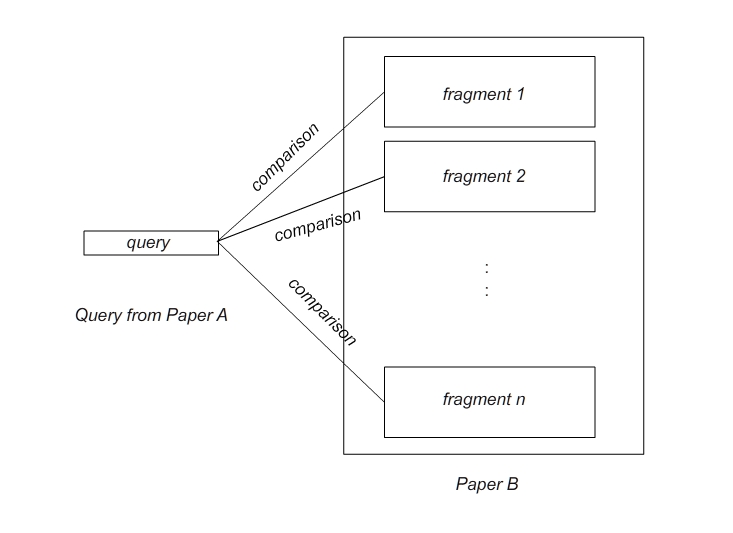
\includegraphics[scale=0.50]{./model}
  \caption{Modeling Our Problem}
  \label{fig:model}
\end{figure}

Our problem is now a \textit{binary classification problem}, where we attempt to determine whether a fragment is either General or Specific.

\section{Building Our Corpus}
\label{buildingcorpus}
At this initial stage, I picked the ACL Anthology Reference Corpus\footnote{http://acl-arc.comp.nus.edu.sg/} (ACL-ARC). The ACL-ARC consists of publications of the Computational Linguistics field. Note that in general, we wish to perform this citation provenance task on all publications from all fields of research. This corpus is chosen as a start, because it provides the \textit{interlink data} that conveniently informs us of the cite links between the papers in the corpus. For instance, in the interlink data, a link like \url{X98-103==>X96-1049} says that the paper \url{X98-103}\footnote{All ACL-ARC papers are assigned an unique paper ID} cites \url{X96-1049}.

Now that I have modelled our problem, I am able to specify the required data format for the task. For each cite link, there can be multiple in-line citations i.e. multiple citing contexts. Each citing context is compared with every fragment in the cited paper. In other words, if a cite link has $n$ citing contexts and the cited paper can be divided into $m$ fragments, immediately we have $(n \times m)$ data instances.

\subsection*{Collecting Annotations - First Attempt}
The first attempt at collecting annotations was to require an annotator to specify the line numbers of the cited information that the citing context was referring to. The annotator would be provided the citing and cited paper in plain text format, and he/she will need to annotate on a separate file, specifying the line number range, e.g. line range \url{L12-55} of the cited paper. For this annotation task, I designed an annotation framework\footnote{http://citprov.heroku.com} where an annotator is presented with an user-friendly interface to select the lines in the cited paper that he/she deem Specific. We posted this task onto the Amazon Mechanical Turk (MTurk\footnote{https://www.mturk.com}) as an attempt to collect annotations on a larger scale and I collected some annotations from a few MTurk workers. After a trial round of annotation, I reviewed this annotation scheme together with feedbacks from the small group of participants.

First, this annotation task is a non-trivial one. Participants must be able to understand the contents of the papers, thus, must be researchers or have some experience in reading scientific papers. While it is possible to target a selected category of MTurk workers for this task, the complexity of this task requires participants with research experiences, which could be limited in numbers. Furthermore, most of the annotations collected from MTurk do not agree among the annotators and ourselves. Thus I abandoned collecting annotations via MTurk, and performed annotations manually.

Second, this annotation scheme is too tricky, and would also cause us much problem when it comes to evaluation. Consider an implemented system that outputs a prediction for citation provenance in the form of a line number range. It is difficult to judge the correctness of this prediction, say \url{L50-78}, when compared against the annotated \url{L12-55}. The prediction \textit{overlaps} the annotation by 5 lines, but this variable amount of overlap is not definitive and difficult to decide at what extent of overlap only do we consider the prediction correct. Thus I switched to the alternative.

\subsection*{Collection Annotations - Second Attempt}
The second attempt is more straightforward. Recall that I use ParsCit for extracting the citing context. ParsCit also divides a paper into logically adequate fragments according to sections, sub-sections, figures and tables etc. So instead of annotating the papers in plain text format by line number ranges, I annotated the structured output from ParsCit, each of the fragments of the cited papers with 3 classes: General ($g$), Specific-Yes ($y$) and Specific-No ($n$). To be precise, I annotate $g$ (for all its fragments) if a cite link is deemed General, and $y$ \underline{only} for the fragment(s) that is deemed Specific. For the other fragments that are not Specific, I annotate $n$. Table \ref{tab:annotation} summarises the statistics for annotation. Note that only percentage values for Specific instances are displayed.

\begin{table}[h]
	\center
	\begin{tabular}{ l | l}
		\textsc{Item} & \textsc{Statistics}\\
		\hline
		No. of Cite Links & 275 (7.6\% Specific) \\
		No. of Fragments & 30943 (0.09\% Specific-Yes, 12.9\% Specific-No)
	\end{tabular}
	\caption{Annotation Statistics}
	\label{tab:annotation}
\end{table}

Specific citations are very rare. From a machine learning point of view, one can observe that the training data is heavily skewed towards General citations. After prolonged periods of searching for valid Specific citations in our training corpus, I argue that despite more attempts to gather more positive instances, the ratio between General and Specific would remain the same. This challenging situation we have with the annotations also contributes to my approach to the problem, as I explain in the following chapter.

During the annotation process, I observed that Specific citations can be categorised into 4 sub-classes. Note, however, these observations are for this particular corpus I worked with. Specific citations may:
\begin{enumerate}
\item refer to digits/numerical figures in the cited paper, usually in the evaluation section
\item refer to term definitions by the author(s) of the cited paper
\item refer to algorithms/theorems in the cited paper
\item quote a line or segment in the cited paper
\end{enumerate}
These observations also led to the implementation of some features that are defined next chapter in my approach.

\chapter{Approach}
\label{approach}
We propose a two-tier approach to our problem. In the first tier, it plays the role of a \textit{filter}, and attempts to filter out the General citations, leaving behind the Specific citations to be passed to the second tier. Figure \ref{fig:twotier} illustrates the flow of our approach.
\begin{figure}[h]
  \centering
  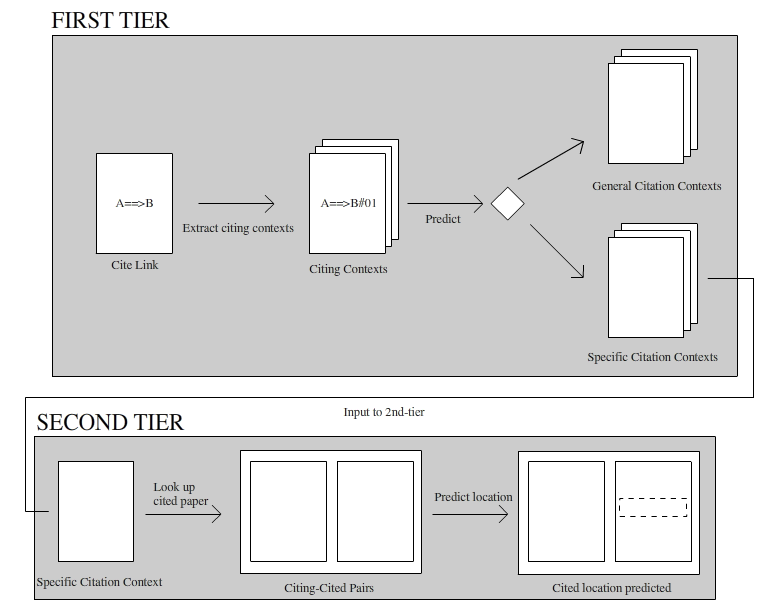
\includegraphics[scale=0.60]{./twotier}
  \caption{A Two-Tier Approach}
  \label{fig:twotier}
\end{figure}

\section{{\it GvS} (First Tier)}
\label{firsttier}
{\it GvS}, short for General versus Specific, is the first tier in our approach to filter out the General citations. In {\it GvS}, we are performing a 2-class \textit{citation classification} task, which already is a challenging task in the research area of citation analysis. We are not interested in determining whether the citation is one of the 12 class as defined by \cite{teufel2009annotation}, but only whether it is General or Specific. {\it GvS} makes use of information only from the citing contexts in a citing paper. We built a model based on features extracted from the citing contexts. With this model, {\it GvS} classifies citing contexts into one of the two classes. Only those contexts that are classified as Specific will be passed to the second tier.

\subsection*{Building The Model For {\it GvS}}
To build a model to classify General versus Specific, we adopt some of the features that \outcite{dongensemble} used for citation classification. From each of the 275 annotated cite links mentioned in Table \ref{tab:annotation} we extracted a set of features into a {\it feature vector} and map it to its {\it label} according to annotation (Figure \ref{fig:featurevector}). The features used are as described below.

\begin{figure}[h]
\centering
$v_1:[f_1, f_2, f_3, \ldots, f_n] \rightarrow L_1$ \\
$v_2:[f_1, f_2, f_3, \ldots, f_n] \rightarrow L_2$ \\
$\vdots$ \\
$v_i:[f_1, f_2, f_3, \ldots, f_n] \rightarrow L_i$ \\
$\vdots$ \\
$v_m:[f_1, f_2, f_3, \ldots, f_n] \rightarrow L_m$
\caption{Mapping feature vectors to labels from annotation}
\label{fig:featurevector}
\end{figure}

\subsection*{{\it GvS} Features}
\begin{enumerate}
\item Physical Features (Feature $A$)\\
We adopted the physical features as presented in \cite{dongensemble}. They are:
\begin{enumerate}
\item \textit{Location}: in which section the citing sentence is from.
\item \textit{Popularity}: no. of citation marks in the citing sentence.
\item \textit{Density}: no. of unique citation marks in the citing sentence and its neighbour sentences.
\item \textit{AvgDens}: the average of Density among the citing and neighbour sentences.
\end{enumerate}
The intuition for using this feature is: A higher number of citation marks within a citing sentence suggests these citations are likely to be General since there was little room of discussion by the author(s).

\item Number Density (Feature $B$)\\
A numerical feature similar to the first feature set that measures the density of numerical figures in the citing context. The intuition is that Specific citations tend refer numerical figures in evaluation results in the cited paper. E.g. ``...Nivre and Scholz (2004) obtained a precision of 79.1\%...". This feature was added based on the observations we made earlier in Chapter \ref{buildingcorpus}.

\item Publishing Year Difference (Feature $C$)\\
A numerical feature that represents difference in the publishing year between the citing and cited paper. The intuition is that higher difference suggests cited paper is older and presented a fundamental idea, and thus cited for General purposes.

\item Citing Context's Average \url{tf-idf} Weight (Feature $D$)\\
A numerical feature that indicates the average amount of \textit{valuable} words, as determined by \url{tf-idf} \cite{irtextbook},  in the citing context. Higher values suggest important words and thus specific keywords.

\item Cue Words (Feature $E$)\\
Another numerical feature adopted from \outcite{dongensemble}, that computes the amount of cue words that appear in the citing sentence and its neighbour sentences. We defined 2 classes of cue words: Cue-General and Cue-Specific (refer to Appendix \ref{cuewords} for list of cue words). These cue words are hand-picked based on the examples we observed during the annotation process.
\end{enumerate}

Recall that according to our annotation statistics, this task is heavily skewed towards General citations. Building a model based on this skewed set of data instances will only produce a bias model that often predicts General. In fact, during some preliminary experiments where all data instances are fitted into the model, it outputs General for all its predictions. To fix this problem, we proposed training the model on {\it unskewed data}.

From the set of labelled feature vectors, we first gathered the Specific instances. Then we {\bf randomly} selected from the rest to have a $1:1$ of Specific vs General instances. While this ratio appear unrealistic compared to the actual statistics, we argue that we am building a model using balanced data to measure its ability to differentiate between the 2 types of citation.

\section{{\it LocateProv} (Second Tier)}
\label{secondtier}
{\it LocateProv}, short for Locate Provenance, is the second tier of my approach. The design of {\it LocateProv} is all its inputs are Specific citations predicts which of the fragments in the cited paper is the cited fragment. Resembling a search, in {\it LocateProv} the citing context becomes the {\it query} to match the cited fragments in the cited paper. For that we also added some features that are common in Information Retrieval tasks.

\subsection*{Building The Model For {\it LocateProv}}
In {\it LocateProv} we are predicting which cited fragment is the provenance of a citation. Instead of cite links, we used the annotated fragments in Table \ref{tab:annotation} to build the model. In this tier the features used are based on both the citing contexts and the cited fragments in order to {\it connect} the citation to its provenance. Similarly the feature vectors are mapped onto the annotated labels.

\subsection*{{\it LocateProv} Features}
\begin{enumerate}
\item Surface Matching (Feature $F$)\\
A numerical feature that measures the amount of word overlap between the citing sentence and a fragment in the cited paper.

\item Number Near-Miss (Feature $G$)\\
A numerical feature that measures the amount of numerical figures overlap between the citing sentence and a fragment in the cited paper. This feature will preprocess each fragment, rounding numerical figures or converting to percentage values when it tries to match the numerical figures in the citing sentence. This feature was added because of the observations we made earlier in Chapter \ref{buildingcorpus}, that citations may refer to evaluation results in the cited paper.

\item Bigrams Matching (Feature $H$)\\
A numerical feature that measures the amount of bigrams overlap between the citing sentence and a fragment in the cited paper. This feature was added to preserve word order when comparing the citing sentence and the fragment. This feature was also targeted at Specific citations that refer to term definitions or quote directly.

\item Cosine Similarity (Feature $I$)\\
A common numerical feature used in Information Retrieval tasks to measure similarity between the query and a candidate document. In our case, citing sentence and the fragment.
\end{enumerate}
Most of these features are added based on some of the observations we made during the annotation tasks.

Again, recall that the data instances that were annotated are heavily skewed against Specific citations. In fact, the ratio of Specific-Yes instances compared to the rest is at least $1:1000$. It is impossible to train a model that is not bias with this entire set of instances. Hence we used the same method used in {\it GvS}: to use a $1:1$ of Specific-Yes versus Specific-No instances. Note that this also coincide with the design of {\it LocateProv} that inputs are only Specific citations. It was also not feasible to use the actual ratio between Specific-Yes and Specific-No because comparing a citing-cited pair of papers, the ratio of citing context to the number of fragments in the cited paper is easily $1:100$.

For both tiers, we trained the models using various classifiers and evaluated their performances on a few evaluation strategies. We discuss the evaluation process in the following chapter.
\chapter{Evaluation}
\label{evaluation}
I performed modular evaluation on {\it GvS} and {\it LocateProv}. For each tier I evaluated its performance on a few classifiers: Support Vector Machine (SVM), Naive Bayes (NB) and Decision Tree (DT). For each classifier I also performed evaluation using a few evaluation strategies.

\section{Evaluating {\it GvS}}
\label{eval:first}
Recall that I used a $1:1$ of Specific versus General data instances for building the model. To first verify {\it GvS}, I evaluated the features added using the {\it feature ablation} strategy. For each feature removed from this set of unskewed data instances, the rest of the features are used to train a model using the SVM classifier and then tested on the same set of data instances. To measure the performance each round, I used the conventional accuracy measure. Note that in Figure \ref{fig:ablation_first} the letters $A$ to $E$ represents the five features described in Chapter \ref{firsttier}.

\begin{figure}[ht]
\begin{minipage}[b]{0.45\linewidth}\centering
\begin{tabular}{ l | l }
Configuration & Accuracy \\
\hline
Full		& 0.911 \\
Full - A	& 0.714 \\
Full - B	& 0.875 \\
Full - C	& 0.786 \\
Full - D	& 0.911 \\
Full - E	& 0.732 \\
\end{tabular}
\end{minipage}
\hspace{0.5cm}
\begin{minipage}[b]{0.45\linewidth}\centering
\begin{tabular}{ c | l }
Configuration & Accuracy \\
\hline
Only A	& 0.696 \\
Only B	& 0.589 \\
Only C	& 0.625 \\
Only D	& 0.535 \\
Only E	& 0.696 \\
\end{tabular}
\end{minipage}
\caption{Feature Ablation on {\it GvS}}
\label{fig:ablation_first}
\end{figure}

We observe that feature $A$ (Physical Feature) has the most impact in the accuracy of the predictions, with the greatest drop in accuracy when $A$ itself is removed and one of the highest accuracy when $A$ alone is used as a feature (see Figure \ref{fig:ablation_first}). Feature $D$ (Citing Context's Average \url{tf-idf} Weight) appears to be the only redundant feature, but since it does not decrease the overall accuracy we shall include it nevertheless.

I first evaluated {\it GvS} using the \url{Leave-One-Out} cross-validation strategy. In this strategy we leave one data instance out for testing while the rest are used for training and we repeat this for the number of instances. The main reason for using this strategy is because the number of data instances in the unskewed data set is already very small, and I wish to maximise them for training. For this strategy I compare the performance of the various classifiers, for each, computing the Precision, Recall and F$_1$ values.

\begin{table}[h]
	\center
	\begin{tabular}{ c | c  c  c | c c c | c c c}
		& & SVM & & & NB & & & DT \\
		\textsc{Class/Values} & \textsc{P} & \textsc{R} & \textsc{F$_1$} & \textsc{P} & \textsc{R} & \textsc{F$_1$} & \textsc{P} & \textsc{R} & \textsc{F$_1$} \\
		\hline
		\textsc{general} 			& 0.76  &    0.79   &   0.77 & 0.64   &   0.82   &   0.72 & 0.67  &    0.64  &    0.65 \\
		\textsc{specific} 			& 0.78  &    0.75   &   0.76 & 0.75   &   0.54   &   0.63 & 0.66  &    0.68  &    0.67 \\
	\end{tabular}
	\caption{Leave-One-Out Results for {\it GvS}}
	\label{tab:firsttieresults}
\end{table}

Let us examine the confusion matrix for the best performing SVM classifier that I ran for the \url{Leave-One-Out} strategy. {\it GvS} is aimed at filtering out the General citations. Our goal is to attain higher numbers in both the $g$-$g$ and $s$-$s$ cells in the confusion matrix. We achieved this in Table \ref{tab:firstsvmconfusionmatrix} and we can conclude that {\it GvS} has a promising performance in differentiating General and Specific citations.

\begin{table}[h]
	\center
	\begin{tabular}{ c | c  c }
		 & \textsc{actual $g$} & \textsc{actual $s$} \\
		\hline
		\textsc{predicted $g$} 	& 22 & 6 \\
		\textsc{predicted $s$}		& 7 & 21
	\end{tabular}
	\caption{Confusion Matrix for SVM with Leave-One-Out on {\it GvS}}
	\label{tab:firstsvmconfusionmatrix}
\end{table}

I continue evaluated {\it GvS} using another cross-validation strategy, $K$-fold. While this appears to be a repeat usage of a cross-validation strategy for evaluation, I wanted to gain a better insight of {\it GvS}'s performance when given less 

%For a more conclusive evaluation, I compared {\it GvS} to my baseline for this task. With {\it GvS} resembling a search problem, a feasible baseline is to compare the citing context with the fragments with Cosine Similarity, coupled with \url{tf-idf} \cite{irtextbook} weighting scheme. Essentially the baseline is just {\it GvS} running only on feature $I$ (Cosine Similarity). For a fair comparison between {\it LocaGvSteProv} and the baseline, I prepared a $1:1$ (Specific-No vs. Specific-Yes) training dataset as I did before to unskew the data instances. Specific-Yes instances were gathered, and the same number of Specific-No instances were {\bf randomly} selected from the collection. For both {\it GvS} and baseline, they were trained and tested on their own data set with the SVM classifier. Note that the only difference between the data set is the random set of Specific-No instances. I compared their P/R/F values in Table \ref{tab:locateprov_vs_baseline}.

\section{Evaluating {\it LocateProv}}
\label{eval:second}
Similar to evaluating {\it GvS} in Chapter \ref{eval:first}, I first evaluate the features added to {\it LocateProv} using the {\it feature ablation} strategy. Note that the letters $F$ to $I$ represents the features described in Chapter \ref{secondtier}.

\begin{figure}[ht]
\begin{minipage}[b]{0.45\linewidth}\centering
\begin{tabular}{ l | l }
Configuration & Accuracy \\
\hline
Full		& 0.893 \\
Full - F	& 0.893 \\
Full - G	& 0.875 \\
Full - H	& 0.893 \\
Full - I	& 0.786 \\
\end{tabular}
\end{minipage}
\hspace{0.5cm}
\begin{minipage}[b]{0.45\linewidth}\centering
\begin{tabular}{ c | l }
Configuration & Accuracy \\
\hline
Only F	& 0.714 \\
Only G	& 0.625 \\
Only H	& 0.607 \\
Only I	& 0.875 \\
\end{tabular}
\end{minipage}
\caption{Feature Ablation on {\it LocateProv}}
\label{fig:ablation_second}
\end{figure}
From Figure \ref{fig:ablation_second} we can conclude that feature $I$ (Cosine Similarity) remains to be the most important among the features for {\it LocateProv}. This is expected because as modelled in Chapter \ref{problemanalysis}, {\it LocateProv} is a searching problem, thus an Information Retrieval solution is most suitable. Note that, however, these results is only this particular test set, which is also the training set. We cannot conclude that Cosine Similarity will work well in all cases.

Again, I continue to evaluate {\it LocateProv} using the \url{Leave-One-Out} strategy together with various classifiers. Table \ref{tab:secondtieresults} summarises the results.

\begin{table}[h]
	\center
	\begin{tabular}{ c | c  c  c | c c c | c c c}
		& & SVM & & & NB & & & DT \\
		\textsc{Class/Values} & \textsc{P} & \textsc{R} & \textsc{F$_1$} & \textsc{P} & \textsc{R} & \textsc{F$_1$} & \textsc{P} & \textsc{R} & \textsc{F$_1$} \\
		\hline
		\textsc{Specific-No} 			& 0.92  &    0.82   &   0.87 & 0.84   &   0.96   &   0.90 & 0.89  &    0.89  &    0.89 \\
		\textsc{Specific-Yes} 			& 0.84  &    0.93   &   0.88 & 0.96   &   0.82   &   0.88 & 0.89  &    0.89  &    0.89 \\
	\end{tabular}
	\caption{Leave-One-Out Results for {\it LocateProv}}
	\label{tab:secondtieresults}
\end{table}
The scores are very close to each other between the classifiers. Let us examine the confusion matrix from the Naive Bayes classifier, which has the highest precision for classifying Specific-Yes instances.

\begin{table}[h]
	\center
	\begin{tabular}{ c | c  c }
		 & \textsc{actual $n$} & \textsc{actual $y$} \\
		\hline
		\textsc{predicted $n$} 	& 27 & 1 \\
		\textsc{predicted $y$}		& 5 & 23
	\end{tabular}
	\caption{Confusion Matrix for NB with Leave-One-Out on {\it LocateProv}}
	\label{tab:secondnbconfusionmatrix}
\end{table}
{\it LocateProv} is aimed at identifying the Specific-Yes fragments in the cited paper. Our goal is to attain higher numbers in both the $g$-$g$ and $s$-$s$ cells in the confusion matrix. We achieved this in Table \ref{tab:secondnbconfusionmatrix} and we can conclude that {\it LocateProv} has a promising performance in differentiating Specific-Yes ($y$) and Specific-No ($n$) fragments.

For a more conclusive evaluation, I compared {\it LocateProv} to my baseline for this task. With {\it LocateProv} resembling a search problem, a feasible baseline is to compare the citing context with the fragments with Cosine Similarity, coupled with \url{tf-idf} \cite{irtextbook} weighting scheme. Essentially the baseline is just {\it LocateProv} running only on feature $I$ (Cosine Similarity). For a fair comparison between {\it LocateProv} and the baseline, I prepared a $1:1$ (Specific-No vs. Specific-Yes) training dataset as I did before to unskew the data instances. Specific-Yes instances were gathered, and the same number of Specific-No instances were {\bf randomly} selected from the collection. For both {\it LocateProv} and baseline, they were trained and tested on their own data set with the SVM classifier. Note that the only difference between the data set is the random set of Specific-No instances. I compared their P/R/F values in Table \ref{tab:locateprov_vs_baseline}.

\begin{table}[h]
	\center
	\begin{tabular}{ c | c  c  c | c c c }
		& & {\it LocateProv} & & & Baseline \\
		\textsc{Class/Values} & \textsc{P} & \textsc{R} & \textsc{F$_1$} & \textsc{P} & \textsc{R} & \textsc{F$_1$}  \\
		\hline
		\textsc{Specific-No} 			& 0.96  &    0.82   &   0.88 & 0.89   &   0.57   &   0.70 \\
		\textsc{Specific-Yes} 			& {\bf 0.84}  &    0.96   &   0.90 & {\bf 0.61}   &   0.89   &   0.72 \\
	\end{tabular}
	\caption{{\it LocateProv} versus Baseline}
	\label{tab:locateprov_vs_baseline}
\end{table}
Notice the precision values in bold in Table \ref{tab:locateprov_vs_baseline}, that {\it LocateProv} is able to perform significantly better than the baseline. Thus, justifying my approach to locating Specific-Yes fragments in the cited paper.
\chapter{Discussion}
\label{discussion}
Citation Provenance is a task that has little developments done on it. In this paper we defined the nature of the problem, and presented a possible approach to tackle it. One of the main challenges we had with this task is the limited number of Specific citations in scientific papers. \outcite{teufel2009annotation} showed that the percentage of neutral citations was 62.7\%. We can say that the percentage of General citations is at least as much, because our definition of a Specific citation is more restricted compared to the 12 classes defined by \outcite{teufel2009annotation}. This supports our observations during annotation collection that most citations are mere {\it mentions}.

We argue that even though the percentage of Specific citations is low and that the value of applications that perform such task seems low, citation provenance would prove to be an important reading tool that helps readers understand and navigate between papers that are linked via citations. we support with evidence the validity of our claim, that a prototype application (that performs Citation Provenance) submitted as part of the \url{Code For Science}\footnote{http://www.codeforscience.com/singapore} 2012 competition organised by Elsevier was well received among the judging panel that consisted of professionals from fields related to information technology and libraries.

Sometimes, in-line citations to scientific papers in journals and books capture the chapter numbers and page numbers. The main reason is because the length of the cited document is very long compared to the citing document. An example of such citation is \textit{(J. Doe, 2012, sec. 6.5, 174-85)}. In this citation it captures the section number, ``\textit{sec. 6.5}", and page numbers, ``\textit{174-85}", to a book or journal. Note that the granularity of such style is not specific enough for our problem as a section can be arbitrary lengthy. In our case, we consider computational linguistic papers that are usually less than 20 pages, which is much shorter than books and journals. For this we sketch a new citation style that better captures citation provenance.

Our sketched style is straightforward: To numerically label each segment or fragment in the cited paper. This applies to text bodies, figures and tables. An example for a Specific citation: \textit{(B. White, 2011, \textbf{B23})}. Notice we added another a \textbf{B} to \textbf{23}, which could be a better way to distinguish between text bodies (B), figures (F) and tables (T). \textbf{23} simply means the 23rd segment of the type B. Suppose the cited paper is already labelled, when a reader sees a citation a paper, the reader sees there is the additional information at the end of the citation and understands it is a Specific citation. To read up on the cited paper would be a breeze.
\chapter{Conclusion}
\label{conclusion}
We touched on a new task for citation analysis, Citation Provenance. While \outcite{csibs} presented the CSIBS tool that gave readers a preview of a cited paper, it only provided a summarisation solution. In our paper, we described the first attempt to provide a solution to the difficulty of locating the information that justifies a citation.

We presented a two-tier approach towards this problem, {\it Gvs} and {\it LocateProv}. With the first acting as a filter to separate the General citations from the Specific ones and the second one to predict which of the fragments in the cited paper are referenced by the citation. One of the challenges in this task is the highly unbalanced ratio between General versus Specific citations. Also, the annotation task is very challenging and would require experienced researchers who understands the content of the papers to be annotated. As a result all the training instances were manually annotated.

To train prediction models for this task, we gathered an unskewed set of instances, a balanced ratio of General versus Specific instances, and measured their ability to differentiate between the 2 types of citations. Feature analysis showed that most of the features are essential, with the Physical Features (Feature $A$) adopted from \outcite{dongensemble} proving to have the most discriminative power in {\it GvS}, and Cosine Similarity (a common strategy for Information Retrieval tasks) remained to be most important in {\it LocateProv}.

Finally, evaluations on {\it GvS} and {\it LocateProv} produced promising results in classifying General versus Specific citations and locating the cited fragment in the cited paper. 

\bibliographystyle{socreport}
\bibliography{bibsource}
\appendix
\chapter{Cue Words}
\label{cuewords}
The following is the list of cue words used in one of our feature. During feature extraction, all words are stemmed before we make any comparison.
\section{Cue-General}
proposed, propose, presented, present, suggested, suggests, described, describe, discuss, discussed, gave, introduction, introduced, shown, showed, sketched, sketch, talked, adopted, adopt, based, originated, originate, built, researchers, comparative, comparison, following, previously, previous

\section{Cue-Specific}
obtains, obtained, score, scored, high, F-score, Precision, precision, Recall, recall, estimated, estimates, reported, reports, probability, probabilities, peaked, experimental, experimented, rate, error

\chapter{Results Details ( {\it GvS} )}
\label{resultsdetails}
\section{Results: Leave-One-Out}
\begin{table}[ht]
\begin{minipage}[b]{0.45\linewidth}\centering
\begin{tabular}{ c | c  c  c }
	& \textsc{Precision} & \textsc{Recall} & \textsc{F$_1$-Score} \\
	\hline
	\textsc{$g$} 	& 0.76  &    0.79   &   0.77 \\
	\textsc{$s$}	& 0.78  &    0.75   &   0.76
\end{tabular}
\end{minipage}
\hspace{0.5cm}
\begin{minipage}[b]{0.45\linewidth}\centering
\begin{tabular}{ c | c  c }
	 & \textsc{actual $g$} & \textsc{actual $s$} \\
	\hline
	\textsc{predicted $g$} 	& 22 & 6 \\
	\textsc{predicted $s$}		& 7 & 21
\end{tabular}
\end{minipage}
\caption{SVM $P/R/F_1$ Scores and Confusion Matrix}
\end{table}

\begin{table}[ht]
\begin{minipage}[b]{0.45\linewidth}\centering
\begin{tabular}{ c | c  c  c }
	& \textsc{Precision} & \textsc{Recall} & \textsc{F$_1$-Score} \\
	\hline
	\textsc{$g$} 	& 0.64  &    0.82   &   0.72 \\
	\textsc{$s$}	& 0.75  &    0.54   &   0.63
\end{tabular}
\end{minipage}
\hspace{0.5cm}
\begin{minipage}[b]{0.45\linewidth}
\centering
\begin{tabular}{ c | c  c }
	 & \textsc{actual $g$} & \textsc{actual $s$} \\
	\hline
	\textsc{predicted $g$} 	& 23 & 5 \\
	\textsc{predicted $s$}		& 13 & 15
\end{tabular}
\end{minipage}
\caption{Naive Bayes $P/R/F_1$ Scores and Confusion Matrix}
\end{table}

\begin{table}[ht]
\begin{minipage}[b]{0.45\linewidth}\centering
\begin{tabular}{ c | c  c  c }
	& \textsc{Precision} & \textsc{Recall} & \textsc{F$_1$-Score} \\
	\hline
	\textsc{$g$} 	& 0.67   &   0.64   &   0.65 \\
	\textsc{$s$}	& 0.66   &   0.68   &   0.67
\end{tabular}
\end{minipage}
\hspace{0.5cm}
\begin{minipage}[b]{0.45\linewidth}
\centering
\begin{tabular}{ c | c  c }
	 & \textsc{actual $g$} & \textsc{actual $s$} \\
	\hline
	\textsc{predicted $g$} 	& 18 & 10 \\
	\textsc{predicted $s$}		& 9 & 19
\end{tabular}
\end{minipage}
\caption{Decision Tree $P/R/F_1$ Scores and Confusion Matrix}
\end{table}
\newpage

%\section{Results: n-Fold}
%\begin{table}[ht]
%\begin{minipage}[b]{0.45\linewidth}\centering
%\begin{tabular}{ c | c  c  c }
%	& \textsc{Precision} & \textsc{Recall} & \textsc{F$_1$-Score} \\
%	\hline
%	\textsc{$g$} 	& 0.76 & 0.57 & 0.65 \\
%	\textsc{$s$}	& 0.66 & 0.82 & 0.73
%\end{tabular}
%\end{minipage}
%\hspace{0.5cm}
%\begin{minipage}[b]{0.45\linewidth}
%\centering
%\begin{tabular}{ c | c  c }
%	 & \textsc{actual $g$} & \textsc{actual $s$} \\
%	\hline
%	\textsc{predicted $g$} 	& 16 & 12 \\
%	\textsc{predicted $s$}		& 5 & 23
%\end{tabular}
%\end{minipage}
%\caption{SVM $P/R/F_1$ Scores and Confusion Matrix}
%\end{table}
%
%\begin{table}[ht]
%\begin{minipage}[b]{0.45\linewidth}\centering
%\begin{tabular}{ c | c  c  c }
%	& \textsc{Precision} & \textsc{Recall} & \textsc{F$_1$-Score} \\
%	\hline
%	\textsc{$g$} 	& 0.61 & 0.89 & 0.72 \\
%	\textsc{$s$}	& 0.80 & 0.43 & 0.56
%\end{tabular}
%\end{minipage}
%\hspace{0.5cm}
%\begin{minipage}[b]{0.45\linewidth}
%\centering
%\begin{tabular}{ c | c  c }
%	 & \textsc{actual $g$} & \textsc{actual $s$} \\
%	\hline
%	\textsc{predicted $g$} 	& 25 & 3 \\
%	\textsc{predicted $s$}		& 16 & 12
%\end{tabular}
%\end{minipage}
%\caption{Naive Bayes $P/R/F_1$ Scores and Confusion Matrix}
%\end{table}
%
%\begin{table}[ht]
%\begin{minipage}[b]{0.45\linewidth}\centering
%\begin{tabular}{ c | c  c  c }
%	& \textsc{Precision} & \textsc{Recall} & \textsc{F$_1$-Score} \\
%	\hline
%	\textsc{$g$} 	& 0.66 & 0.68 & 0.67 \\
%	\textsc{$s$}	& 0.67 & 0.64 & 0.65
%\end{tabular}
%\end{minipage}
%\hspace{0.5cm}
%\begin{minipage}[b]{0.45\linewidth}
%\centering
%\begin{tabular}{ c | c  c }
%	 & \textsc{actual $g$} & \textsc{actual $s$} \\
%	\hline
%	\textsc{predicted $g$} 	& 19 & 9 \\
%	\textsc{predicted $s$}		& 10 & 18
%\end{tabular}
%\end{minipage}
%\caption{Decision Tree $P/R/F_1$ Scores and Confusion Matrix}
%\end{table}



\chapter{Results Details ( {\it LocateProv} )}
\section{Results: Leave-One-Out}
\begin{table}[ht]
\begin{minipage}[b]{0.45\linewidth}\centering
\begin{tabular}{ c | c  c  c }
	& \textsc{Precision} & \textsc{Recall} & \textsc{F$_1$-Score} \\
	\hline
	\textsc{$n$} 	& 0.92  &    0.82   &   0.87 \\
	\textsc{$y$}	& 0.84  &    0.93   &   0.88
\end{tabular}
\end{minipage}
\hspace{0.5cm}
\begin{minipage}[b]{0.45\linewidth}
\centering
\begin{tabular}{ c | c  c }
	 & \textsc{actual $n$} & \textsc{actual $y$} \\
	\hline
	\textsc{predicted $n$} 	& 23 & 5 \\
	\textsc{predicted $y$}		& 2 & 26
\end{tabular}
\end{minipage}
\caption{SVM $P/R/F_1$ Scores and Confusion Matrix}
\end{table}

\begin{table}[ht]
\begin{minipage}[b]{0.45\linewidth}\centering
\begin{tabular}{ c | c  c  c }
	& \textsc{Precision} & \textsc{Recall} & \textsc{F$_1$-Score} \\
	\hline
	\textsc{$n$} 	& 0.84   &   0.96   &   0.90 \\
	\textsc{$y$}	& 0.96   &   0.82   &   0.88
\end{tabular}
\end{minipage}
\hspace{0.5cm}
\begin{minipage}[b]{0.45\linewidth}
\centering
\begin{tabular}{ c | c  c }
	 & \textsc{actual $n$} & \textsc{actual $y$} \\
	\hline
	\textsc{predicted $n$} 	& 27 & 1 \\
	\textsc{predicted $y$}		& 5 & 23
\end{tabular}
\end{minipage}
\caption{Naive Bayes $P/R/F_1$ Scores and Confusion Matrix}
\end{table}

\begin{table}[ht]
\begin{minipage}[b]{0.45\linewidth}\centering
\begin{tabular}{ c | c  c  c }
	& \textsc{Precision} & \textsc{Recall} & \textsc{F$_1$-Score} \\
	\hline
	\textsc{$n$} 	& 0.89   &   0.89   &   0.89 \\
	\textsc{$y$}	& 0.89   &   0.89   &   0.89
\end{tabular}
\end{minipage}
\hspace{0.5cm}
\begin{minipage}[b]{0.45\linewidth}
\centering
\begin{tabular}{ c | c  c }
	 & \textsc{actual $n$} & \textsc{actual $y$} \\
	\hline
	\textsc{predicted $n$} 	& 25 & 3 \\
	\textsc{predicted $y$}		& 3 & 25
\end{tabular}
\end{minipage}
\caption{Decision Tree $P/R/F_1$ Scores and Confusion Matrix}
\end{table}
\newpage

%\section{Results: n-Fold}
%\begin{table}[ht]
%\begin{minipage}[b]{0.45\linewidth}\centering
%\begin{tabular}{ c | c  c  c }
%	& \textsc{Precision} & \textsc{Recall} & \textsc{F$_1$-Score} \\
%	\hline
%	\textsc{$g$} 	& 0.91 & 0.71 & 0.80 \\
%	\textsc{$s$}	& 0.76 & 0.93 & 0.84
%\end{tabular}
%\end{minipage}
%\hspace{0.5cm}
%\begin{minipage}[b]{0.45\linewidth}
%\centering
%\begin{tabular}{ c | c  c }
%	 & \textsc{actual $g$} & \textsc{actual $s$} \\
%	\hline
%	\textsc{predicted $g$} 	& 20 & 8 \\
%	\textsc{predicted $s$}		& 2 & 26
%\end{tabular}
%\end{minipage}
%\caption{SVM $P/R/F_1$ Scores and Confusion Matrix}
%\end{table}
%
%\begin{table}[ht]
%\begin{minipage}[b]{0.45\linewidth}\centering
%\begin{tabular}{ c | c  c  c }
%	& \textsc{Precision} & \textsc{Recall} & \textsc{F$_1$-Score} \\
%	\hline
%	\textsc{$g$} 	& 0.73 & 0.86 & 0.79 \\
%	\textsc{$s$}	& 0.83 & 0.68 & 0.75
%\end{tabular}
%\end{minipage}
%\hspace{0.5cm}
%\begin{minipage}[b]{0.45\linewidth}
%\centering
%\begin{tabular}{ c | c  c }
%	 & \textsc{actual $g$} & \textsc{actual $s$} \\
%	\hline
%	\textsc{predicted $g$} 	& 24 & 4 \\
%	\textsc{predicted $s$}		& 9 & 19
%\end{tabular}
%\end{minipage}
%\caption{Naive Bayes $P/R/F_1$ Scores and Confusion Matrix}
%\end{table}
%
%\begin{table}[ht]
%\begin{minipage}[b]{0.45\linewidth}\centering
%\begin{tabular}{ c | c  c  c }
%	& \textsc{Precision} & \textsc{Recall} & \textsc{F$_1$-Score} \\
%	\hline
%	\textsc{$g$} 	& 0.88 & 0.82 & 0.85 \\
%	\textsc{$s$}	& 0.83 & 0.89 & 0.86
%\end{tabular}
%\end{minipage}
%\hspace{0.5cm}
%\begin{minipage}[b]{0.45\linewidth}
%\centering
%\begin{tabular}{ c | c  c }
%	 & \textsc{actual $g$} & \textsc{actual $s$} \\
%	\hline
%	\textsc{predicted $g$} 	& 23 & 5 \\
%	\textsc{predicted $s$}		& 3 & 25
%\end{tabular}
%\end{minipage}
%\caption{Decision Tree $P/R/F_1$ Scores and Confusion Matrix}
%\end{table}

\end{document}
